\documentclass[tikz]{article}
\usepackage[utf8]{inputenc}
\usepackage[tmargin=2in]{geometry}
\usepackage{setspace}
\usepackage{verbatim}
\usepackage{listings}
\usepackage{amsmath}
\usepackage{amssymb}
\usepackage{pgfplots}
\usepackage{graphics}
\usepackage{csvsimple}
\usepackage{array}
\usepackage{longtable}
\usepackage{booktabs}
\usepackage{pgfplotstable}
\usepackage[toc,page]{appendix}
\usepackage{indentfirst}
\usepackage{float}
\usepackage{setspace}
\usetikzlibrary{positioning}

\doublespacing
\pagenumbering{gobble}

\pgfplotsset{every axis/.style={scale only axis}}

\begin{document}

\begin{center}
Dustin McAfee \\
Project 5 Report \\
Fall 2018 \\
\end{center}

\singlespacing

\section{Objective}
\label{sec:obj}
There are three datasets for use with (soft-margin) Support Vector Machines (SVMs) in classification. The first is a binary classification problem: predicting 'good' or 'bad' interactions of radar signals with electrons in the ionosphere. This dataset has 351 instances and 34 attributes. The second classification is multi-class with 11 classes: predicting vowels independent of the speaker. This dataset has 528 instances and 10 attributes. The last classification problem is also multi-class with 7 classes: predicting terrain type from multi-spectral values of pixels in 3 by 3 neighborhoods in satellite images. This dataset has 4435 training observations and 2000 testing instances with 36 features. The objective is to perform grid searches on SVMs with different kernels (linear, polynomial, radial basis), each with different hyper-parameters in order to find an optimal SVM (with optimal hyper-parameters) for each dataset.

\section{Methods}
\label{sec:methods}
A Support Vector Machine (SVM) is a supervised machine learning algorithm which can be used for both classification or regression. In this scope, SVM is used for classification, and in this respect, (soft-max) SVM minimizes the error of classification by creating boundaries (discriminants) between classes, with specified slack to the boundary. The slack variables allow for non-separable categories of data: If the data is non-separable, then the slack variables need to be increased, which allows for categorization of observations that are just passed the discriminant hyperplane. The kernel of this algorithm is, essentially, the shape of the hyperplane that defines the discriminant. With a linear kernel, the hyperplane is linear. Polynomial hyperplanes (polynomial kernels) take a hyper-parameter that is the degree of the polynomial. The Radial Basis Kernel is a distance measure of the observation to a center point. In this paper, the radial basis kernel used is Gaussian, and so the distances are measured in a Gaussian probability curve, which acts as a similarity measure. The objective of the SVM is to maximize the distance of each point from each discriminant hyper-plane, while minimizing the error. Increasing the complexity factor (hyper-parameter for each kernel) decreases the margin for the discriminant hyper-plane, making it more specific to the current training dataset, potentially over-fitting the data. On the other hand, a small complexity factor results in large margins for the discriminant hyper-plane, which allows for more noise (higher slack variables). The mathematics for this is shown below.

A linear discriminant hyperplane can be written as the set of points \textbf{x} satisfying \\
\begin{align*}
\mathbf{w} \cdot \mathbf{x}^{t} + w_{0} = 0
\end{align*}
The boundaries of this hyperplane (with a distance of 1 from the discriminant) can be written as the set of points \textbf{x} satisfying \\
\begin{align*}
\mathbf{w} \cdot \mathbf{x}^{t} + w_{0} = 1 \text{ and } \mathbf{w} \cdot \mathbf{x}^{t} + w_{0} = -1
\end{align*}
To maximize these margins, $\frac{2}{||\mathbf{w}||^{2}}$ needs to be maximized, which means $||\mathbf{w}||$ needs to be minimized. To minimize error, we need to minimize the number of data points that fall past the margin of the discriminant. If $r^{t}(\mathbf{w} \cdot \mathbf{x}^{t} + w_{0}) \geq 1$ is a 'hard' constraint (no observations are allowed past the margins), then $r^{t}(\mathbf{w} \cdot \mathbf{x}^{t} + w_{0}) \geq 1 - \xi^{t}$ is a 'soft' margin, in which $\xi^{t}$ represents the slack variable corresponding to observation $\mathbf{x}^{t}$. To this end, the hinge loss function is introduced:
\begin{align*}
\xi^{t} = \max(0, 1 - r^{t}(\mathbf{w} \cdot \mathbf{x}^{t} + w_{0})),
\end{align*}
which is zero if the observation obeys the hard constraint. For observations that do not obey the hard margin, the value is proportional to the distance from the margin. The goal, then, is to
\begin{align*} 
\text{minimize: } \frac{1}{2}||\mathbf{w}||^{2} + C\sum_{t} \xi^{t} \\
\text{subject to: } r^{t}(\mathbf{w} \cdot \mathbf{x}^{t} + w_{0}) \geq 1 - \xi^{t},
\end{align*}
where $C$ is the complexity factor (otherwise known as penalty). This is also known as the primal problem, and by solving for the Lagrangian dual of this problem obtains the simpler problem:
\begin{gather*}
\text{maximize: } \sum_{t}\alpha^{t} - \frac{1}{2}\sum_{t}\sum_{s}\alpha^{t}\alpha^{s}r^{t}r^{s}(\mathbf{x}^{t} \cdot \mathbf{x}^{s}) \\
\text{subject to: } \sum_{t}\alpha^{t}r^{t} = 0, \\ 
\text{and } 0 \leq \alpha^{t} \leq \frac{1}{n}
\end{gather*}
The dot product between the two observations, $\mathbf{x}^{t}$ and $\mathbf{x}^{s}$ is called a linear kernel, because it describes a linear discriminant hyper-plane. A polynomial kernel expands the feature-set to include higher order terms before making the dot product, and the radial basis kernel uses the function, $e^{-\gamma||\mathbf{x}^{t} - \mathbf{x}^{s}||^{2}}$, where $\gamma > 0$ is a hyper-parameter for this specific kernel. A small gamma means a Gaussian discriminant hyper-plane with a large variance, which means the influence of $\mathbf{x}^{s}$ is large (vice versa for large gamma).

\section{Data Preprocessing}
\label{sec:preprocessing}
Each dataset is z-normalized, and the attributes scaled in the range of [0,1]. There are no missing values in the three datasets, but the categorical attribute for the ionosphere dataset (binary) is converted to 0/1 and separated into a testing dataset (20\% or 70 observations), and a training dataset (281 observations). K-fold cross-validation is performed with 3 folds on the training dataset of the ionospheric data. For the vowel dataset, 20\% is separated for the testing dataset (198 observations), and for the satellite image dataset, the testing dataset comes pre-separated with about 31\% of the data (2000 observations). For the satellite and vowel dataset, K-fold cross-validation is performed with 6 folds.

\begin{comment}
TODO: Add info on preprocessing of other 2 datasets
\end{comment}

\section{Training Results}
\label{sec:res_tr}
K-fold cross-validation is used for validation of hyper-parameters. For each classification problem, a coarse grid search is performed for the hyper-parameters of the polynomial kernel (degree and $C$ complexity factor) and for the hyper-parameters of the radial basis kernel ($\gamma$ and $C$). A fine grid search is then performed for the kernel than performs better, and the optimal hyper-parameters are chosen from the fine grid searches. The fine grid search is ran in the 'neighborhoods' of the optimal hyper-parameters chosen from the coarse grid search. The kernel that yields the best results is chosen to run with its optimal hyper-parameters on the testing dataset. For coarse grid searches, the complexity factor, $C$, is tested from the range of 0.0001 to 100000, by factors of 10, and gamma is tested (in the radial basis kernel) in the same range of $C$. For the polynomial kernel, the degree hyper-parameter is tested from 1 to 5.

\subsection{Ionospheric Dataset}
\label{sec:ionosphere}
For this binary classification problem, the discriminant hyper-plane is determined from the only two possible classes (one vs one only). The K-fold cross-validation mean accuracy and precision measurements from the coarse grid search using a polynomial kernel (See file "output/ionosphere/ionosphere\_train\_poly.txt") are shown below, in Figure \ref{fig:ion_poly_1}. The 95\% confidence interval is also given for these performance measurements.

\begin{figure}[H]
\centering
\begin{tabular}{|c|c|c|c|}
\hline
Hyper-Parameter $C$ & Hyper-Parameter degree & Mean Accuracy & Mean Precision \\
\hline
$\leq$0.1 & - & 0.637 $\pm$ 0.002 & 0.637 $\pm$ 0.002 \\
\hline
1 & 1 & 0.797 $\pm$ 0.023 & 0.759 $\pm$ 0.021 \\
\hline
1 & 2 & 0.829 $\pm$ 0.053 & 0.791 $\pm$ 0.054 \\
\hline
1 & 3 & 0.699 $\pm$ 0.127 & 0.683 $\pm$ 0.096 \\
\hline
1 & 4 & 0.637 $\pm$ 0.002 & 0.637 $\pm$ 0.002 \\
\hline
1 & 5 & 0.637 $\pm$ 0.002 & 0.637 $\pm$ 0.002 \\
\hline
10 & 1 & 0.922 $\pm$ 0.018 & 0.905 $\pm$ 0.026 \\
\hline
10 & 2 & 0.929 $\pm$ 0.010 & 0.919 $\pm$ 0.018 \\
\hline
10 & 3 & 0.929 $\pm$ 0.018 & 0.921 $\pm$ 0.024 \\
\hline
10 & 4 & 0.927 $\pm$ 0.014 & 0.921 $\pm$ 0.024 \\
\hline
10 & 5 & 0.907 $\pm$ 0.022 & 0.917 $\pm$ 0.032 \\
\hline
100 & 1 & 0.964 $\pm$ 0.005 & 0.954 $\pm$ 0.019 \\
\hline
100 & 2 & 0.979 $\pm$ 0.018 & 0.976 $\pm$ 0.034 \\
\hline
100 & 3 & 0.974 $\pm$ 0.015 & 0.978 $\pm$ 0.028 \\
\hline
100 & 4 & 0.968 $\pm$ 0.023 & 0.978 $\pm$ 0.028 \\
\hline
100 & 5 & 0.961 $\pm$ 0.013 & 0.975 $\pm$ 0.014 \\
\hline
1000 & 1 & 0.989 $\pm$ 0.005 & 0.986 $\pm$ 0.015 \\
\hline
1000 & 2 & 0.996 $\pm$ 0.005 & 0.994 $\pm$ 0.008 \\
\hline
1000 & 3 & 0.996 $\pm$ 0.005 & 0.994 $\pm$ 0.008 \\
\hline
1000 & 4 & 0.991 $\pm$ 0.013 & 0.992 $\pm$ 0.013 \\
\hline
1000 & 5 & 0.984 $\pm$ 0.015 & 0.992 $\pm$ 0.014 \\
\hline
10000 & 1 & 0.998 $\pm$ 0.005 & 0.997 $\pm$ 0.008 \\
\hline
$\geq$10000 & $\geq$2 & 1 $\pm$ 0 & 1 $\pm$ 0  \\
\hline
\end{tabular}
\caption{Polynomial SVM Performance with Ionospheric Data}
\label{fig:ion_poly_1}
\end{figure}

These same performance measurements are shown, again, for a radial basis kernel SVM, below, in Figure \ref{fig:ion_rbf_1}.
\begin{figure}[H]
\centering
\begin{tabular}{|c|c|c|c|}
\hline
Hyper-Parameter $C$ & Hyper-Parameter $\gamma$ & Mean Accuracy & Mean Precision \\
\hline
0.1 & $\leq$0.01 & 0.637 $\pm$ 0.002 & 0.637 $\pm$ 0.002 \\
\hline
0.1 & 0.1 & 0.653 $\pm$ 0.022 & 0.647 $\pm$ 0.014 \\
\hline
0.1 & 1 & 0.847 $\pm$ 0.245 & 0.824 $\pm$ 0.230 \\
\hline
0.1 & $\geq$10 & 0.637 $\pm$ 0.002 & 0.637 $\pm$ 0.002 \\
\hline
1 & $\leq$0.001 & 0.637 $\pm$ 0.002 & 0.637 $\pm$ 0.002 \\
\hline
1 & 0.01 & 0.714 $\pm$ 0.024 & 0.690 $\pm$ 0.017 \\
\hline
1 & 0.1 & 0.943 $\pm$ 0.018 & 0.918 $\pm$ 0.024 \\
\hline
1 & 1 & 0.991 $\pm$ 0.010 & 0.992 $\pm$ 0.013 \\
\hline
$\geq$1 & $\geq$10 & 1 $\pm$ 0 & 1 $\pm$ 0  \\
\hline
\end{tabular}
\caption{Radial Basis Function SVM Performance with Ionospheric Data}
\label{fig:ion_rbf_1}
\end{figure}

The hyper-parameter selected should give the best generalization of the data. Of course, high complexity factor $C$ means less generalization properties of the classifying discriminant hyper-plane. In other words, with large $C$, the SVM tries to fit the data as best as possible with little slack. To this end, the optimal hyper-parameter intervals chosen for the fine grid search are from the radial basis SVM, which has better generalization than the polynomial SVM. A finer grid search is run for the chosen $C$ = 1 hyper-parameter, and $\gamma \in \{0.05, 0.1, 0.15, 0.2, 0.3, 0.4, 0.5, 0.6, 0.7, 0.8, 0.9, 1\}$, and the average accuracy and precision for the K-fold cross-validation is shown, below, in Figure \ref{fig:ion_rbf_2}.
\begin{figure}[H]
\centering
\begin{tabular}{|c|c|c|c|}
\hline
Hyper-Parameter $C$ & Hyper-Parameter $\gamma$ & Mean Accuracy & Mean Precision \\
\hline
1 & 0.05 & 0.915 $\pm$ 0.027 & 0.882 $\pm$ 0.033 \\
\hline
1 & 0.1 & 0.943 $\pm$ 0.018 & 0.918 $\pm$ 0.024 \\
\hline
1 & 0.15 & 0.952 $\pm$ 0.009 & 0.934 $\pm$ 0.018 \\
\hline
1 & 0.2 & 0.966 $\pm$ 0.010 & 0.955 $\pm$ 0.019 \\
\hline
1 & 0.3 & 0.975 $\pm$ 0.005 & 0.970 $\pm$ 0.008 \\
\hline
1 & 0.4 & 0.980 $\pm$ 0.005 & 0.978 $\pm$ 0.008 \\
\hline
1 & 0.5 & 0.984 $\pm$ 0.009 & 0.983 $\pm$ 0.013 \\
\hline
1 & 0.6 & 0.984 $\pm$ 0.009 & 0.983 $\pm$ 0.013 \\
\hline
1 & 0.7 & 0.986 $\pm$ 0.005 & 0.986 $\pm$ 0.008 \\
\hline
1 & 0.8 & 0.989 $\pm$ 0.009 & 0.989 $\pm$ 0.008 \\
\hline
1 & 0.9 & 0.991 $\pm$ 0.010 & 0.992 $\pm$ 0.013 \\
\hline
1 & 1 & 0.991 $\pm$ 0.010 & 0.992 $\pm$ 0.013 \\
\hline
\end{tabular}
\caption{Radial Basis Function SVM Performance with Ionospheric Data}
\label{fig:ion_rbf_2}
\end{figure}
A decent elbow point for both the mean accuracy and mean precision of the K-fold cross-validation seems to be at $\gamma = 0.7$ from $C = 1$. These are run on the testing dataset, with the confusion matrix shown below, in Figure \ref{fig:ion_test}.

\begin{figure}[H]
\begin{center}
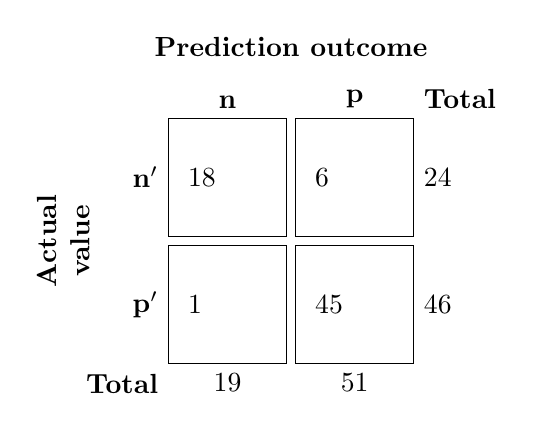
\begin{tikzpicture}[
box/.style={draw,rectangle,minimum size=1.5cm,text width=1.0cm,align=left}]
\matrix (conmat) [row sep=.1cm,column sep=.1cm] {
\node (tneg) [box,
    label=left:\( \mathbf{n'} \),
    label=above:\( \mathbf{n} \),
    ] {18};
&

\node (fpos) [box,
    label=above:\textbf{p},
    label=above right:\textbf{Total},
    label=right:\( \mathrm{24} \)] {6};
\\
\node (fneg) [box,
    label=left:\( \mathbf{p'} \),
    label=below left:\textbf{Total},
    label=below:19] {1};
&
\node (tpos) [box,
    label=right:\( \mathrm{46} \),
    label=below:51] {45};
\\
};
\node [rotate=90,left=.05cm of conmat,anchor=center,text width=1.5cm,align=center] {\textbf{Actual \\ value}};
\node [above=.05cm of conmat] {\textbf{Prediction outcome}};
\end{tikzpicture}
\caption{Confusion Matrix for Testing Dataset: Radial Basis SVM; $\gamma = 0.7$; $C = 1$}
\label{fig:ion_test}
\end{center}
\end{figure}
This yields 90\% accuracy and 88.2\% precision. The precision is lower than expected (higher false positive rate), seeing as though the training set had an average of 0.986\% precision and accuracy.

\subsection{Vowel Dataset}
\label{sec:vowel}
For this multi-class classification problem, the discriminant hyper-plane is determined from the multiple classes using OVA (one versus all). The K-fold cross-validation mean AUC ROC (Area Under Curve Receiver Operating Characteristics) and precision measurements from the coarse grid search using a polynomial kernel (See file "output/vowels/vowels\_train\_poly.txt") are shown below, in Figure \ref{fig:vowel_poly_1}. The 95\% confidence interval is also given for these performance measurements. The ROC is a probability curve, and AUC represents a measurement of separability.

\begin{figure}[H]
\centering
\begin{tabular}{|c|c|c|c|}
\hline
Hyper-Parameter $C$ & Hyper-Parameter degree & Mean ROC AUC & Mean Precision \\
\hline
$\leq$ 100 & $\leq$ 5 & 0.651 $\pm$ 0.009 & 0.301 $\pm$ 0.026 \\
\hline
1000 & 1 & 0.623 $\pm$ 0.010 & 0.281 $\pm$ 0.021 \\
\hline
1000 & 2 & 0.821 $\pm$ 0.007 & 0.640 $\pm$ 0.020 \\
\hline
1000 & 3 & 0.797 $\pm$ 0.007 & 0.602 $\pm$ 0.015 \\
\hline
1000 & 4 & 0.730 $\pm$ 0.016 & 0.490 $\pm$ 0.029 \\
\hline
1000 & 5 & 0.653 $\pm$ 0.012 & 0.359 $\pm$ 0.026 \\
\hline
10000 & 1 & 0.626 $\pm$ 0.009 & 0.286 $\pm$ 0.021 \\
\hline
10000 & 2 & 0.959 $\pm$ 0.006 & 0.897 $\pm$ 0.015 \\
\hline
10000 & 3 & 0.961 $\pm$ 0.004 & 0.908 $\pm$ 0.014 \\
\hline
10000 & 4 & 0.941 $\pm$ 0.009 & 0.872 $\pm$ 0.016 \\
\hline
10000 & 5 & 0.879 $\pm$ 0.007 & 0.755 $\pm$ 0.011 \\
\hline
100000 & 1 & 0.626 $\pm$ 0.010 & 0.285 $\pm$ 0.021 \\
\hline
$\geq$ 100000 & $\geq$ 2 & $\geq$ 0.991 & $\geq$ 0.969 \\
\hline
\end{tabular}
\caption{Polynomial SVM Performance with Vowel Data}
\label{fig:vowel_poly_1}
\end{figure}

This dataset seems to have the worst performance when attempted to separate the classes linearly (degree = 1). Furthermore, the SVM (with polynomial kernel) only performs well for extremely large $C$ values, which is bad generalization. These same performance measurements are shown, again, for a radial basis kernel SVM, below, in Figure \ref{fig:vowel_rbf_1}.

\begin{figure}[H]
\centering
\begin{tabular}{|c|c|c|c|}
\hline
Hyper-Parameter $C$ & Hyper-Parameter $\gamma$ & Mean ROC AUC & Mean Precision \\
\hline
$\leq$ 1 & $\leq$ 1 & $\leq$ 0.636  & $\leq$ 0.334 \\
\hline
1 & 10 & 0.992 $\pm$ 0.004 & 0.984 $\pm$ 0.007 \\
\hline
1 & $\geq$ 100 & 1.0 $\pm$ 0.0 & 1.0 $\pm$ 0.0 \\
\hline
10 & $\leq$ 0.1 & $\leq$ 0.597 & $\leq$ 0.253 \\
\hline
10 & 1 & 0.921 $\pm$ 0.009 & 0.831 $\pm$ 0.012 \\
\hline
10 & $\geq$ 10 & 1.0 $\pm$ 1.0 & 1.0 $\pm$ 1.0 \\
\hline
100 & $\leq$ 0.1 & $\leq$ 0.718 & $\leq$ 0.458 \\
\hline
100 & 1 & 0.997 $\pm$ 0.001 & 0.989 $\pm$ 0.005 \\
\hline
100 & $\geq$ 10 & 1.0 $\pm$ 0.0 & 1.0 $\pm$ 0.0 \\
\hline
1000 & $\leq$ 0.01 & $\leq$ 0.630 & $\leq$ 0.298 \\
\hline
1000 & 0.1 & 0.920 $\pm$ 0.010 & 0.821 $\pm$ 0.018 \\
\hline
1000 & $\geq$ 1 & 1.0 $\pm$ 0.0 & 1.0 $\pm$ 0.0 \\
\hline
10000 & $\leq$ 0.01 & $\leq$ 0.722 & $\leq$ 0.461 \\
\hline
10000 & 0.1 & 0.989 $\pm$ 0.007 & 0.965 $\pm$ 0.012 \\
\hline
10000 & $\geq$ 1 & 1.0 $\pm$ 0.0 & 1.0 $\pm$ 0.0 \\
\hline
10000 & $\leq$ 0.001 & $\leq$ 0.637 & $\leq$ 0.310 \\
\hline
10000 & 0.01 & 0.916 $\pm$ 0.011 & 0.811 $\pm$ 0.018 \\
\hline
10000 & $\geq$ 0.1 & 1.0 $\pm$ 0.0 & 1.0 $\pm$ 0.0 \\
\hline
\end{tabular}
\caption{Radial Basis Function SVM Performance with Vowel Data}
\label{fig:vowel_rbf_1}
\end{figure}

Likewise from Section \ref{sec:ionosphere}, a low $C$ is chosen for the fine grid search. Specifically, the fine grid search is for $C \in \{1, 2, 3, 4, 5, 6, 7, 8\}$, and $\gamma \in \{1, 2, 3, 4, 5, 6, 7, 8\}$. Most of these results are omitted here, since there are exactly 64 instances to look through (See file "output/vowels/vowels\_train\_rbf\_fine.txt"). Because of this, only the relevant results are shown, below in Figure \ref{fig:vowel_rbf_2}, of which, the optimal hyper-parameters are chosen.

\begin{figure}[H]
\centering
\begin{tabular}{|c|c|c|c|}
\hline
Hyper-Parameter $C$ & Hyper-Parameter $\gamma$ & Mean ROC AUC & Mean Precision \\
\hline
1 & 4 & 0.915 $\pm$ 0.008 & 0.840 $\pm$ 0.017 \\
\hline
1 & 5 & 0.945 $\pm$ 0.010 & 0.898 $\pm$ 0.019 \\
\hline
1 & 6 & 0.964 $\pm$ 0.007 & 0.934 $\pm$ 0.013 \\
\hline
1 & 7 & 0.975 $\pm$ 0.006 & 0.954 $\pm$ 0.012 \\
\hline
1 & 8 & 0.984 $\pm$ 0.004 & 0.970 $\pm$ 0.009 \\
\hline
2 & 3 & 0.947 $\pm$ 0.009 & 0.894 $\pm$ 0.019 \\
\hline
2 & 4 & 0.973 $\pm$ 0.003 & 0.948 $\pm$ 0.009 \\
\hline
2 & 5 & 0.989 $\pm$ 0.008 & 0.977 $\pm$ 0.016 \\
\hline
2 & 6 & 0.995 $\pm$ 0.005 & 0.989 $\pm$ 0.008 \\
\hline
2 & 7 & 0.997 $\pm$ 0.003 & 0.993 $\pm$ 0.005 \\
\hline
2 & 8 & 0.998 $\pm$ 0.002 & 0.995 $\pm$ 0.004 \\
\hline
3 & 2 & 0.924 $\pm$ 0.008 & 0.848 $\pm$ 0.013 \\
\hline
3 & 3 & 0.971 $\pm$ 0.006 & 0.940 $\pm$ 0.012 \\
\hline
3 & 4 & 0.990 $\pm$ 0.006 & 0.978 $\pm$ 0.011 \\
\hline
3 & $\geq$ 5 & $\geq$ 0.996 & $\geq$ 0.991 \\
\hline
4 & 2 & 0.947 $\pm$ 0.006 & 0.891 $\pm$ 0.012 \\
\hline
4 & 3 & 0.984 $\pm$ 0.006 & 0.964 $\pm$ 0.012 \\
\hline
4 & $\geq$ 4 & $\geq$ 0.995 & $\geq$ 0.988 \\
\hline
5 & 2 & 0.960 $\pm$ 0.006 & 0.916 $\pm$ 0.010 \\
\hline
5 & 3 & 0.991 $\pm$ 0.005 & 0.979 $\pm$ 0.010 \\
\hline
5 & $\geq$ 4 & $\geq$ 0.997 & $\geq$ 0.992 \\
\hline
6 & 2 & 0.970 $\pm$ 0.007 & 0.936 $\pm$ 0.011 \\
\hline
6 & $\geq$ 3 & $\geq$ 0.993 & $\geq$ 0.984 \\
\hline
7 & 2 & 0.977 $\pm$ 0.008 & 0.948 $\pm$ 0.015 \\
\hline
7 & $\geq$ 3 & $\geq$ 0.995 & $\geq$ 0.988 \\
\hline
8 & 1 & 0.901 $\pm$ 0.003 & 0.795 $\pm$ 0.009 \\
\hline
8 & 2 & 0.982 $\pm$ 0.006 & 0.958 $\pm$ 0.010 \\
\hline
8 & $\geq$ 3 & $\geq$ 0.996 & $\geq$ 0.990 \\
\hline
\end{tabular}
\caption{Radial Basis Function SVM Performance with Vowel Data}
\label{fig:vowel_rbf_2}
\end{figure}
$C$ and $\gamma$ are chosen low, but not too low as to lower precision. A good elbow point is $C = 2$ and $\gamma = 5$, where their performance scores tend to level off after increasing any more. The precision for execution of the SVM (with Radius Basis kernel) with the chosen optimal hyper-parameters is 0.942, and the ROC AUC is 0.976, which is comparable to the training dataset. This means that this SVM is likely a good generalization for this dataset.

\subsection{Satellite Dataset}
\label{sec:sat}
For this multi-class classification problem, the discriminant hyper-plane is determined from the multiple classes using OVA (one versus all). The K-fold cross-validation mean AUC ROC and precision measurements from the coarse grid search using a polynomial kernel (See file "output/sat/sat\_train\_poly.txt") are calculated with 95\% confidence interval. The performance on this dataset for the polynomial kernel is extremely low and omitted here. For execution with the Radial Basis kernel (See file "output/sat/sat\_train\_rbf.txt"), see Figure \ref{fig:sat_rbf_1} below.

\begin{figure}[H]
\centering
\begin{tabular}{|c|c|c|c|}
\hline
Hyper-Parameter $C$ & Hyper-Parameter $\gamma$ & Mean ROC AUC & Mean Precision \\
\hline
$\leq$ 0.1 & - & $\leq$ 0.850 & $\leq$ 0.703 \\
\hline
1 & $\leq$ 0.1 & $\leq$ 0.844 & $\leq$ 0.686 \\
\hline
1 & 1 & 0.917 $\pm$ 0.005 & 0.807 $\pm$ 0.009 \\
\hline
1 & 10 & 0.972 $\pm$ 0.003 & 0.936 $\pm$ 0.006 \\
\hline
1 & $\geq$ 100 & 1.0 $\pm$ 0.0 & 1.0 $\pm$ 0.0 \\
\hline
10 & $\leq$ 0.1 & $\leq$ 0.868 & $\leq$ 0.729 \\
\hline
10 & 1 & 0.952 $\pm$ 0.004 & 0.880 $\pm$ 0.007 \\
\hline
10 & $\geq$ 10 & 1.0 $\pm$ 0.0 & 1.0 $\pm$ 0.0 \\
\hline
100 & $\leq$ 0.01 & $\leq$ 0.852 & $\leq$ 0.699 \\
\hline
100 & 0.1 & 0.923 $\pm$ 0.007 & 0.814 $\pm$ 0.009 \\
\hline
100 & 1 & 0.982 $\pm$ 0.002 & 0.951 $\pm$ 0.005 \\
\hline
100 & $\geq$ 10 & 1.0 $\pm$ 0.0 & 1.0 $\pm$ 0.0 \\
\hline
1000 & $\leq$ 0.01 & 0.878 $\pm$ 0.012 & 0.744 $\pm$ 0.019 \\
\hline
1000 & 0.1 & 0.950 $\pm$ 0.003 & 0.869 $\pm$ 0.007 \\
\hline
1000 & 1 & .999 $\pm$ 0.001 & 0.997 $\pm$ 0.002 \\
\hline
1000 & $\geq$ 10 & 1.0 $\pm$ 0.0 & 1.0 $\pm$ 0.0 \\
\hline
10000 & 0.0001 & 0.817 $\pm$ 0.005 & 0.646 $\pm$ 0.011 \\
\hline
10000 & 0.001 & 0.853 $\pm$ 0.004 & 0.701 $\pm$ 0.009 \\
\hline
10000 & 0.01 & 0.924 $\pm$ 0.009 & 0.813 $\pm$ 0.012 \\
\hline
10000 & 0.1 & 0.971 $\pm$ 0.004 & 0.922 $\pm$ 0.007 \\
\hline
10000 & $\geq$ 1 & 1.0 $\pm$ 0.0 & 1.0 $\pm$ 0.0 \\
\hline
100000 & 0.0001 & 0.831 $\pm$ 0.006 & 0.668 $\pm$ 0.011 \\
\hline
100000 & 0.001 & 0.881 $\pm$ 0.012 & 0.747 $\pm$ 0.017 \\
\hline
100000 & 0.01 & 0.949 $\pm$ 0.004 & 0.863 $\pm$ 0.005 \\
\hline
100000 & 0.1 & 0.994 $\pm$ 0.002 & 0.980 $\pm$ 0.003 \\
\hline
100000 & $\geq$ 1 & 1.0 $\pm$ 0.0 & 1.0 $\pm$ 0.0 \\
\hline
\end{tabular}
\caption{Radial Basis SVM Performance with Satellite Data}
\label{fig:sat_rbf_1}
\end{figure}

$C = 1$ is chosen for the fine grid search, along with $\gamma \in \{8, 9, 10, 11, 12, 13, 14, 15, 20, 25\}$, and the average performance metrics is shown, below, in Figure \ref{fig:sat_rbf_2}.

\begin{figure}[H]
\centering
\begin{tabular}{|c|c|c|c|}
\hline
Hyper-Parameter $C$ & Hyper-Parameter $\gamma$ & Mean ROC AUC & Mean Precision \\
\hline
1 & 8 & 0.967 $\pm$ 0.004 & 0.923 $\pm$ 0.009 \\
\hline
1 & 9 & 0.970 $\pm$ 0.004 & 0.930 $\pm$ 0.008 \\
\hline
1 & 10 & 0.972 $\pm$ 0.004 & 0.936 $\pm$ 0.007 \\
\hline
1 & 11 & 0.974 $\pm$ 0.003 & 0.941 $\pm$ 0.006 \\
\hline
1 & 12 & 0.976 $\pm$ 0.003 & 0.945 $\pm$ 0.006 \\
\hline
1 & 13 & 0.977 $\pm$ 0.003 & 0.949 $\pm$ 0.006 \\
\hline
1 & 14 & 0.979 $\pm$ 0.003 & 0.952 $\pm$ 0.006 \\
\hline
1 & 15 & 0.980 $\pm$ 0.003 & 0.956 $\pm$ 0.005 \\
\hline
1 & 20 & 0.986 $\pm$ 0.002 & 0.968 $\pm$ 0.004 \\
\hline
1 & 25 & 0.990 $\pm$ 0.001 & 0.979 $\pm$ 0.002 \\
\hline
\end{tabular}
\caption{Radial Basis SVM Performance with Satellite Data}
\label{fig:sat_rbf_2}
\end{figure}

There is no extremely obvious elbow point, here. Instead, a 'best guess' is performed here, with $\gamma = 13$, since there seems to be less increase from $\gamma = 12$ to $13$ than from $\gamma = 13$ to $14$. To this end, $C = 1$ and $\gamma = 13$ are chosen to run on the testing dataset. The precision from the execution on the testing dataset is 0.783, and the ROC AUC is 0.891, which implies a better fit (slight over-fit) for the training dataset.


\section{Conclusion}
\label{sec:conclusion}
In general, the Radial Basis kernel SVM has higher performance metrics for lower $C$ values than the polynomial kernel SVM. For the multi-valued categorical datasets, the polynomial kernel does not perform well at all. For the first two datasets (ionosphere dataset and vowel dataset), the hyper-parameters had noticeable elbow points from the grid searches that helps determine the optimal values. Consequently, the execution of the SVM on the testing data with the training data's respective optimal hyper-parameters (from the ionosphere and vowel datasets) yields high performance comparable to the performance of the cross-validation. This indicates a good generalization from the training dataset to the testing dataset. However, the satellite dataset does not have an obvious elbow point in the performance metrics of the cross-validation, which may be the reason the chosen optimal hyper-parameters for this set yields lower performance on the testing dataset than on the cross-validation, indicating an over-fit of the training data.

\end{document}

